\documentclass[10pt]{beamer}

\usepackage{../macros}

\usepackage{pgfplots}
\usepgfplotslibrary{dateplot}

\usepackage{tikz}
\usetikzlibrary{calc, shapes, backgrounds,decorations,arrows,shadows}

\tikzset{%
  box/.style={rectangle,draw=gray, thick, fill=lightgray,minimum size=1cm},
  algo/.style={->, thick, color=red!80},
  sync/.style={dashed, thick, color=blue!80}
}

\tikzset{
  treenode/.style = {align=center, inner sep=0pt, text centered,
    font=\sffamily},
  arn_b/.style = {treenode, circle, black, font=\sffamily\bfseries, draw=black, text width=1.5em, very thick},% noeud noir
  arn_r/.style = {treenode, circle, red, draw=red, 
    text width=1.5em, very thick},% arbre rouge noir, noeud rouge
  arn_x/.style = {treenode, rectangle, draw=black,
    minimum width=0.5em, minimum height=0.5em}% arbre rouge noir, nil
}

\newcommand{\F}[1]{\ensuremath{{\cal F}_{#1}}\xspace}

\title{Suite de Fibonacci}

\hypersetup{
  pdftitle =  {Suite de Fibonacci}
}

\begin{document}

\maketitle

%%%%%%%%%%%%%%%%%%%%%%%%%%%%%%%%%%%%%%%%%%%%%%%%%%%%%%%
\begin{frame}{Suite de Fibonacci}

  \begin{block}{Définition}
    Le $n$-ème terme est défini ainsi :
    \begin{equation*}
      \F{n} = \F{n-1} + \F{n-2}
    \end{equation*}
    et $\F{0} = 0$, $\F{1} = 1$.
  \end{block}
  
  \begin{exampleblock}{Premiers termes}
    0, 1, 1, 2, 3, 5, 8, 13, 21, 34, 55, 89, 144, 233, 377, 610, \dots
  \end{exampleblock}
  \begin{figure}[htbp]
    \centering
    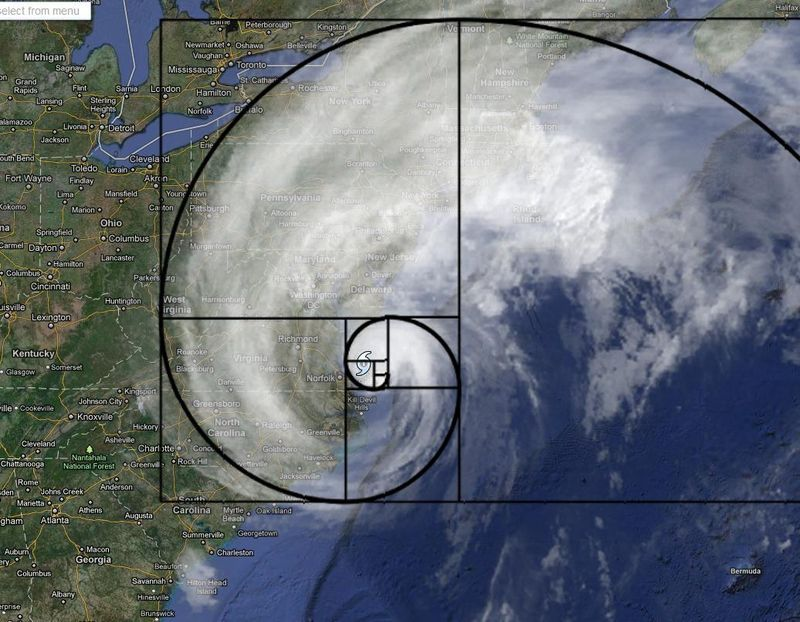
\includegraphics[width=0.42\textwidth]{nuages-parfaits}
    \hfill
    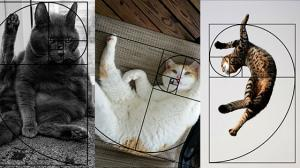
\includegraphics[width=0.42\textwidth]{chats-parfaits}
  \end{figure}
  \href{https://archzine.fr/lifestyle/art/suite-de-fibonacci-harmonieuse/}{D'autres d'images de suites de Fibonacci harmonieuses.}

\end{frame}

%%%%%%%%%%%%%%%%%%%%%%%%%%%%%%%%%%%%%%%%%%%%%%%%%%%%%%%
\begin{frame}[fragile]{Récursion simple (top-down)}

  \begin{lstlisting}[style=editor]
F <- function(n) {
  if( n < 2) return(n)
  else return(F(n-1) + F(n-2))
}
\end{lstlisting}
\begin{center}
  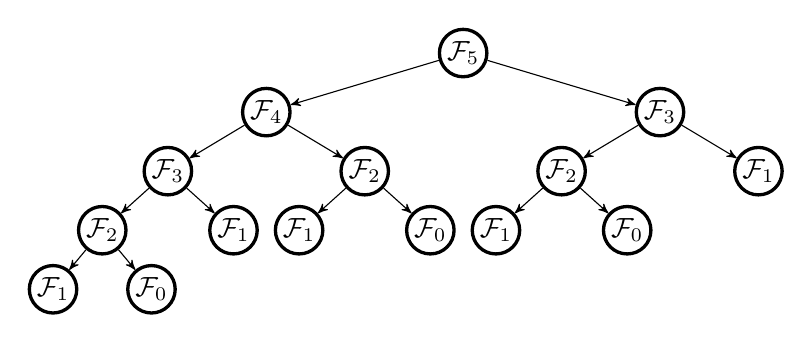
\begin{tikzpicture}[->,>=stealth',level/.style={sibling distance = 5cm/#1, level distance = 0.75cm}] 
    \node [arn_b] {\F{5}} 
    child{ node [arn_b] {\F{4}} 
      child{ node [arn_b] {\F{3}}
        child{ node [arn_b] {\F{2}}
          child{ node [arn_b] {\F{1}}} 
          child{ node [arn_b] {\F{0}}}
        } 
        child{ node [arn_b] {\F{1}}}
      } % edge from parent node[above left] {$x$}} %for a named pointer
      child{ node [arn_b] {\F{2}}
        child{ node [arn_b] {\F{1}}} 
        child{ node [arn_b] {\F{0}}}
      }
    }
    child{ node [arn_b] {\F{3}}
      child{ node [arn_b] {\F{2}}
        child{ node [arn_b] {\F{1}}} 
        child{ node [arn_b] {\F{0}}}
      } 
      child{ node [arn_b] {\F{1}}}
    }                          
    ; 
  \end{tikzpicture}
\end{center}

  \begin{alertblock}{Catastrophe ! La complexité de l'algorithme est exponentielle !}
    Plus de 15 secondes pour calculer F(35) !
  \end{alertblock}

%   \begin{tikzpicture}[->,>=stealth',level/.style={sibling distance = 6cm/#1, level distance = 1cm}] 
%     \node [arn_b] {\F{6}}
%     child{ node [arn_b] {\F{5}} 
%       child{ node [arn_b] {\F{4}} 
%         child{ node [arn_b] {\F{3}}
%           child{ node [arn_b] {\F{2}}
%             child{ node [arn_b] {\F{1}}} 
%             child{ node [arn_b] {\F{0}}}
%           } 
%           child{ node [arn_b] {\F{1}}}
%         } % edge from parent node[above left] {$x$}} %for a named pointer
%         child{ node [arn_b] {\F{2}}
%           child{ node [arn_b] {\F{1}}} 
%           child{ node [arn_b] {\F{0}}}
%         }
%       }
%       child{ node [arn_b] {\F{3}}
%         child{ node [arn_b] {\F{2}}
%           child{ node [arn_b] {\F{1}}} 
%           child{ node [arn_b] {\F{0}}}
%         } 
%         child{ node [arn_b] {\F{1}}}
%       }                          
%     }
%     child{ node [arn_b] {\F{4}} 
%       child{ node [arn_b] {\F{3}}
%         child{ node [arn_b] {\F{2}}
%           child{ node [arn_b] {\F{1}}} 
%           child{ node [arn_b] {\F{0}}}
%         } 
%         child{ node [arn_b] {\F{1}}}
%       } 
%       child{ node [arn_b] {\F{2}}
%           child{ node [arn_b] {\F{1}}} 
%           child{ node [arn_b] {\F{0}}}
%         }
%     }
%  ; 
% \end{tikzpicture}
\end{frame}

%%%%%%%%%%%%%%%%%%%%%%%%%%%%%%%%%%%%%%%%%%%%%%%%%%%%%%%%
\begin{frame}
  \frametitle{Mémo-fonction}
  \alert{Programmer une fonction qui se souvient des calculs déjà effectués !}

  \begin{exampleblock}{Exemple avec Fibonacci}
    \begin{itemize}
    \item Je calcule \F{35} qui demande le calcul de \F{34}.
    \item Je calcule \F{36} qui demande une seule addition \\si je suis capable de me souvenir de \F{35} et de \F{34}.   
    \end{itemize}
  \end{exampleblock}

  \begin{block}{Comment ?}
    \begin{itemize}
    \item Nous allons gérer un dictionnaire privé à la fonction qui va contenir tous les couples n:v tels que \F{n} == v ait déjà été calculé !
    \item Ici, le dictionnaire est un vecteur tel que \F{n} est à la position $n+1$.
      \begin{itemize}
      \item les indices de la suite commencent à 0.
      \item les indices du vecteur commencent à 1.
      \end{itemize}
    \item<alert@1> Le dictionnaire joue le rôle de mémoire cache.
    \end{itemize}
\end{block}



\end{frame}

%%%%%%%%%%%%%%%%%%%%%%%%%%%%%%%%%%%%%%%%%%%%%%%%%%%%%%%%
\begin{frame}[fragile]
  \frametitle{Portée des variables}
Jusqu'à présent, dans plusieurs fonctions, nous avons introduit des variables qui n'étaient pas des paramètres de la fonction, souvent un compteur \texttt{i} ou un accumulateur \texttt{acc}.
\begin{itemize}
\item Une telle variable est dite \alert{locale} à la fonction et n'a rien à voir avec une variable de même nom existant en-dehors de cette fonction !  
\item Une variable définie en-dehors de toute fonction est \alert{globale}.  
\end{itemize}

\begin{lstlisting}
> i <- 42
> foo <- function() {print(i); i <- 33; print(i)}
> foo()
[1] 42 # globale
[1] 33 # locale
> i # globale
[1] 42  
\end{lstlisting}
\begin{itemize}
\item<alert@1> Les modifications apportées à une variable globale sont locales !
\item Conclusion : les variables introduites dans une fonction sont locales !
\item<alert@1> Pourquoi R a-t-il fait ce choix ? Pour décourager autant que possible l'utilisation de variables globales ! Dont acte \dots
\end{itemize}

\end{frame}


%%%%%%%%%%%%%%%%%%%%%%%%%%%%%%%%%%%%%%%%%%%%%%%%%%%%%%%%
\begin{frame}[fragile]
  \frametitle{Modifier quand même une variable globale !}

  \begin{alertblock}{Opérateur \alert{\texttt{<<-}}}
    Les modifications apportées à une variable globale sont globales !
  \end{alertblock}

\begin{lstlisting}
> i <- 42
> foo <- function() {print(i); i <<- 33; print(i)}
> foo()
[1] 42 # Globale.
[1] 33 # Globale aussi. 
> i # Globale toujours !
[1] 33
\end{lstlisting}
\end{frame}



%%%%%%%%%%%%%%%%%%%%%%%%%%%%%%%%%%%%%%%%%%%%%%%%%%%%%%%%
\begin{frame}[fragile]{Mémo-fonction de Fibonacci}

  \begin{lstlisting}[style=editor]
cache <- c(0, 1, 1)
F <- function(n) {
  if(length(cache) <= n) {
    cache[n + 1] <<- F(n-1) + F(n-2)
  }
  return(cache[n + 1]) 
}
\end{lstlisting}



\begin{columns}[c]
\begin{column}{0.45\textwidth}
\begin{lstlisting}
> F(35) # Immédiat !
[1] 9227465
> F(30) 
[1] 832040 # Déjà calculé !
\end{lstlisting}
\end{column}
\begin{column}{0.55\textwidth}
  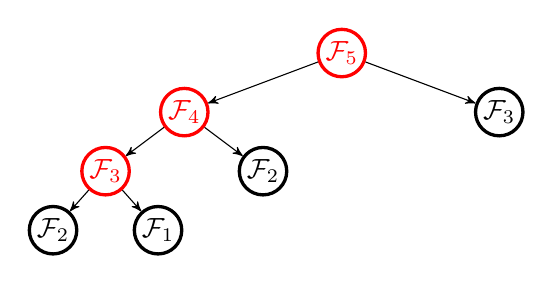
\begin{tikzpicture}[->,>=stealth',level/.style={sibling distance = 4cm/#1, level distance = 0.75cm}] 
    \node [arn_r] {\F{5}} 
    child{ node [arn_r] {\F{4}} 
      child{ node [arn_r] {\F{3}}
        child{ node [arn_b] {\F{2}}} 
        child{ node [arn_b] {\F{1}}}
      } % edge from parent node[above left] {$x$}} %for a named pointer
      child{ node [arn_b] {\F{2}}}
    }
    child{ node [arn_b] {\F{3}}}                          
    ; 
\end{tikzpicture}

\end{column}
\end{columns}

\begin{center}
\end{center}

\begin{alertblock}{Sauvé ! Les complexités temporelles et spatiales sont linéaires !}
  Le calcul de F(35) est immédiat.
\end{alertblock}


\end{frame}

%%%%%%%%%%%%%%%%%%%%%%%%%%%%%%%%%%%%%%%%%%%%%%%%%%%%%%%%
\begin{frame}[fragile]{Limites de la mémo-fonction de Fibonacci}
  
  \begin{exampleblock}{En mettant de côté les dépassements de capacité,}
    \begin{lstlisting}[style=block]
> F(1000)
[1] 4.346656e+208
> F(2000)
[1] Inf
\end{lstlisting}
\end{exampleblock}

\begin{alertblock}{La récursivité pose toujours problème !}
    \begin{lstlisting}[style=block]
> F(10000)
Erreur : C stack usage  7969716 is too close to the limit
    \end{lstlisting}
  \end{alertblock}
\end{frame}

%%%%%%%%%%%%%%%%%%%%%%%%%%%%%%%%%%%%%%%%%%%%%%%%%%%%%%%%
\begin{frame}[fragile]{Mémo-fonction : cacher le cache !}
  \begin{block}{Le cache est public !}
    Modifions le cache juste après la définition de la mémo-fonction.
\begin{lstlisting}
> cache <- c(5, 13, 34)
> F(3)
[1] 47
\end{lstlisting}
\end{block}
\begin{block}{Utilisons un constructeur pour la fonction \texttt{F}}
  Une fonction renvoyant une fonction comme résultat !

\begin{columns}[t]
\begin{column}{0.55\textwidth}
\begin{lstlisting}[style=editor]
MakeF <- function() {
  cache <- c(0, 1, 1)
  F <- function(n) {
    if(length(cache) <= n) {
      cache[n + 1] <<- F(n-1) + F(n-2)
    }
    return(cache[n + 1]) 
  }
  return(F)
}
  \end{lstlisting}
\end{column}
\begin{column}{0.45\textwidth}
  \begin{lstlisting}
> F <- MakeF()
> cache <- c(5, 13, 34)
> F(3)
[1] 2    
  \end{lstlisting}
\end{column}
\end{columns}
\end{block}
\end{frame}


%%%%%%%%%%%%%%%%%%%%%%%%%%%%%%%%%%%%%%%%%%%%%%%%%%%%%%%%
\begin{frame}[fragile]{Suppression de la récursivité (bottom-up)}
  Il faut construire une itération calculant les termes par ordre croissant.
  \begin{alertblock}{Suppression de la récursivité}
    \begin{lstlisting}[style=edblock]
F <- function(n) {
    cache <- c(0, 1, 1)
    if(length(cache) <= n) {
      for(j in seq(from = length(cache) + 1, to = n + 1)) {
        cache[j] <- cache[j-1] + cache[j-2]
      }
    }
    return(cache[n + 1]) 
  }   
    \end{lstlisting}
  \end{alertblock}


  \begin{exampleblock}{Plus de problème avec la pile d'appels}
    \begin{lstlisting}[style=block]
> F(10000)
[1] Inf    
    \end{lstlisting}
  \end{exampleblock}

\end{frame}


%%%%%%%%%%%%%%%%%%%%%%%%%%%%%%%%%%%%%%%%%%%%%%%%%%%%%%%%
\begin{frame}[fragile]{Réduction de la complexité spatiale}
  
    \begin{lstlisting}[style=edblock]
F <- function(n) {
  if(n < 2) return(n)
  x <- c(0, 1) # F(0), F(1)
  i <- 2;
  while(i <= n) {
    x <- c(x[2], sum(x)) # F(n-1), F(n)
    i <- i + 1;
  }
  return(x[2]) 
}
\end{lstlisting}
%
\begin{alertblock}{La complexité spatiale est maintenant constante !}
 
  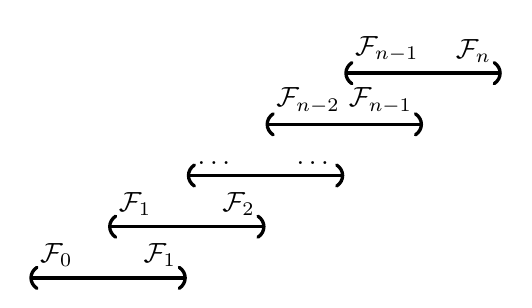
\begin{tikzpicture}
    \draw[(-), very thick] (0,0) node[above right] {\F{0}} -- (2,0) node[above left] {\F{1}};
    \draw[(-), very thick] (1, 0.65) node[above right] {\F{1}} -- (3, 0.65) node[above left] {\F{2}};
    \draw[(-), very thick] (2, 1.3) node[above right] {\dots} -- (4, 1.3) node[above left] {\dots};
    \draw[(-), very thick] (3, 1.95) node[above right] {\F{n-2}} -- (5, 1.95) node[above left] {\F{n-1}};
    \draw[(-), very thick] (4, 2.6) node[above right] {\F{n-1}} -- (6, 2.6) node[above left] {\F{n}};
  \end{tikzpicture}

\end{alertblock}
\end{frame}

%%%%%%%%%%%%%%%%%%%%%%%%%%%%%%%%%%%%%%%%%%%%%%%%%%%%%%%
\begin{frame}[fragile]
  \frametitle{Matrice de Fibonacci }
  \begin{lstlisting}
> library(expm) # pour les puissances de matrice   
> mF <- matrix(c(0, 1, 1, 1), nrow = 2)
\end{lstlisting}
  
\begin{columns}[t]
\begin{column}{0.48\textwidth}
  \begin{lstlisting}
> mF
     [,1] [,2]
[1,]    0    1
[2,]    1    1
> mF %^% 4
     [,1] [,2]
[1,]    2    3
[2,]    3    5
\end{lstlisting}

\end{column}
\begin{column}{0.48\textwidth}
  \begin{lstlisting}
> mF %^% 7
     [,1] [,2]
[1,]    8   13
[2,]   13   21
> mF %^% 10
     [,1] [,2]
[1,]   34   55
[2,]   55   89
\end{lstlisting}

\end{column}
\end{columns}


\begin{block}{Exponentiation rapide}
  Les méthodes d'exponentiation rapide permettent d'atteindre une \alert{complexité logarithmique}.
\end{block}
\end{frame}

%%%%%%%%%%%%%%%%%%%%%%%%%%%%%%%%%%%%%%%%%%%%%%%%%%%%%%%
\questionSlide

%%%%%%%%%%%%%%%%%%%%%%%%%%%%%%%%%%%%%%%%%%%%%%%%%%%%%%%
 \appendix
 \backupSlides
%%%%%%%%%%%%%%%%%%%%%%%%%%%%%%%%%%%%%%%%%%%%%%%%%%%%%%%

%%%%%%%%%%%%%%%%%%%%%%%%%%%%%%%%%%%%%%%%%%%%%%%%%%%%%%%
% \begin{frame}[fragile]{Backup slides}
%   Sometimes, it is useful to add slides at the end of your presentation to
%   refer to during audience questions.

%   The best way to do this is to include the \verb|appendixnumberbeamer|
%   package in your preamble and call \verb|\appendix| before your backup slides.

%   will automatically turn off slide numbering and progress bars for
%   slides in the appendix.
% \end{frame}


%%%%%%%%%%%%%%%%%%%%%%%%%%%%%%%%%%%%%%%%%%%%%%%%%%%%%%%
% \begin{frame}[allowframebreaks]{References}

%   % \bibliography{../bib_parallelism,../bib_others}
%   % \bibliographystyle{abbrv}

% \end{frame}

\end{document}

%%% Local Variables:
%%% mode: latex
%%% TeX-master: t
%%% End:
